\section{Full Financial Audits and Secondary Tests}
\label{sec:supp-financial-audit}

The empirical layer audits ex post whether a financial library can be
compressed without discarding access to useful descendants.  The primary
comparison is innovation-safe versus frontier-only pruning; coverage ranking
is a secondary stress test.  The information-set boundary is summarized in
the main paper's Appendix~E and applies to every definition and result below.
The terminal financial audit is the fixed-split protocol, whereas the annual
walk-forward financial audit is the five-decision protocol.  They are separate
audits with different held-out estimands; neither supersedes the other and
their outcome levels are never pooled.

\subsection{Data, design locks, and resampling}

Both audits use the same licensed CRSP/WRDS snapshot; raw and row-level files
remain nonredistributable.  The fixed daily snapshot covers 2008--2024.  The
terminal audit design locks 25 date-valid surviving ETFs, 2,400 strategies, three
sample splits, 500 seeded circular-block replications with 20-session blocks,
and the 1/5/10-basis-point cost schedule before scoring.  The annual
walk-forward design fixes an outcome-blind 100-ETF manifest, five belief
states, trailing five-year estimation, sequential top-five selection, five
annual targets, 2,000 seeded annual-unit bootstrap replications, and the same
cost schedule.  Signals use information through close \(t\), followed by a
two-return-index lag.  Neither universe is survivorship-free and neither
holdout is prospective.

For each ETF, the fixed grammar enumerates three directional signals and two
choices each of entry filter, horizon, sizing, exit, and risk constraint:
\(3\cdot2^5=96\) policies per instrument, each carrying the resulting seven
modules.  Development is 2009--2014, validation is 2015--2019, and the
held-out period is 2020--2024.  The ignored licensed panels contain 106,975
and 427,900 rows, respectively, each with 4,279 complete common dates.

\subsection{Compression and descendant-quality estimands}
\label{sec:supp-financial-estimands}

Write \(a\in\{\mathrm{T},\mathrm{A}\}\) for the locked terminal and annual
walk-forward audits, \(L_a\) for the source library, \(L_a^F\) for
frontier-only pruning, and \(L_a^S\) for innovation-safe compression.  For
empirical belief cell \(b\), policy payoff \(\widehat j_{ai}(b)\), and fixed
cell weights \(\widehat\mu_a(b)\), define
\begin{align}
  \widehat F_a(b;L')
    &:=\max_{i\in L'}\widehat j_{ai}(b),&
  \overline F_a(L')
    &:=\sum_b\widehat\mu_a(b)\widehat F_a(b;L'),
    \label{eq:supp-financial-frontier}\\
  C_a(L')
    &:=\bigcup_{i\in L'}M(i),&
  r_a(L')
    &:=1-\frac{|L'|}{|L_a|}.
    \label{eq:supp-financial-closure-reduction}
\end{align}
The full frontier vector is computed from validation profiles and is available
to both pruning rules; frontier equality is their common deletion gate.
Module closure is structural information available at the same time and is
the additional innovation-safe gate.  The compression ratio is calculated
only after a pruning run terminates and is a retrospective, outcome-blind
description, not a deletion criterion.

Let \(\mathcal G_a\) be the fixed candidate catalog, \(M(c)\) the modules
required by candidate \(c\), and \(q_a(c)\) its quality measured from held-out
audit outcomes.  Define
\begin{align}
  E_a(L')&:=\{c\in\mathcal G_a:M(c)\subseteq C_a(L')\},\nonumber\\
  Q_a(L')&:=\max_{c\in E_a(L')}q_a(c).
  \label{eq:supp-financial-descendant-quality}
\end{align}
The enabled set \(E_a(L')\) is structurally derivable from the fixed catalog
and closure before the holdout, but neither pruning rule tests candidate-set
equality.  The quantity \(Q_a(L')\), the \emph{ex post enabled-descendant
opportunity quality}, measures whether the modules retained in \(L'\) would
have preserved access to candidates that realized high quality in the held-out
audit.  It is evaluated only after pruning decisions are fixed and is neither
a forecast, a policy score, nor a deployable selection criterion.

For the locked terminal audit, \(q_{\mathrm T}\) is locked-period candidate net
utility.  For the annual walk-forward audit, \(q_{\mathrm A}\) is mean realized
candidate coverage over the five 2020--2024 targets.  Their levels are not
comparable.  The displayed changes are
\[
  \Delta\overline F_a(L'):=\overline F_a(L')-\overline F_a(L_a),
  \qquad
  \Delta Q_a(L'):=Q_a(L')-Q_a(L_a).
\]
At each deletion decision, innovation-safe pruning accepts a removal using
only equality of the current frontier and module closure; it never evaluates
\(Q_a\).  Frontier-only pruning uses frontier equality alone.  Thus
\(\Delta Q_a\) is an ex post mechanism diagnostic, not an allegation that
frontier-only pruning ignored known future outcomes.

\subsection{Deletion-contribution audit}

For policy \(i\) retained in the safe library \(L_a^S\), define the empirical
deletion contributions
\begin{align}
  \widehat O_{ai}
    &:=\widehat P_a(L_a^S)-\widehat P_a(L_a^S\setminus\{i\}),\nonumber\\
  \widehat G_{ai}
    &:={}
      \bigl[\widehat U_a(L_a^S)
       -\widehat U_a(L_a^S\setminus\{i\})\bigr]-\widehat O_{ai},
  \label{eq:supp-financial-policy-contributions}
\end{align}
where \(\widehat P_a\) freezes the library and \(\widehat U_a\) retains the
research option.  The operational-only, generative-only, both, and neither
counts classify the signs of \((\widehat O_{ai},\widehat G_{ai})\).  Frontier
sparsity, module uniqueness, and candidate dependence are
\[
 S_{ai}:=\mathbf 1\{\widehat O_{ai}=0\},\qquad
 H_{ai}:=\frac{1}{|M(i)|}\sum_{m\in M(i)}
   \mathbf 1\!\left\{|\{j\in L_a^S:m\in M(j)\}|=1\right\},
\]
\[
 D_{ai}:=
 |\{c\in\mathcal G_a:
   M(c)\subseteq C_a(L_a^S),\\
   M(c)\nsubseteq C_a(L_a^S\setminus\{i\})\}|.
\]
The full frontier vector is the preservation gate; the main figure reports
its weighted scalar change.  Operational contribution and frontier sparsity
are post-compression, validation-derived descriptions.  Module uniqueness
and descendant dependence are post-compression structural descriptions of the
final safe library and use no held-out outcome.  Generative contribution is
computed from held-out \(Q_a\), and the ``supports best descendant'' flag also
uses the ex post identity of the maximizing candidate.  None of these
policy-characteristic statistics enters pruning.

\subsection{Primary safe-versus-frontier-only audit}

Frontier-only pruning reduces the libraries from \(80\) to \(3\) and from
\(202\) to \(5\).  It leaves every current cell frontier unchanged, yet
\(\Delta Q_{\mathrm T}(L_{\mathrm T}^F)=-0.0016\) and
\(\Delta Q_{\mathrm A}(L_{\mathrm A}^F)=-0.1020\); both changes are ex post.
Innovation-safe compression retains 25 and 100 policies, respectively, and
satisfies
\[
  \widehat F_a(\,\cdot\,;L_a^S)=\widehat F_a(\,\cdot\,;L_a),\qquad
  C_a(L_a^S)=C_a(L_a),\qquad
  Q_a(L_a^S)=Q_a(L_a).
\]
The frontier-only libraries retain 12 of 38 and 14 of 113 source-closure
modules, whereas the innovation-safe closure identities are \(38=38\) and
\(113=113\).  Thus the financial audits show, using held-out outcomes, that
present-frontier preservation alone did not preserve access to the
highest-quality enabled descendants in these two audits.  This diagnostic
statement neither changes either pruning rule nor turns realized quality into
information known at deletion time.

Each safe library has exactly one positive ex post generative carrier: GLD has
\((O,G)=(0,0.0016)\) and UNG has \((O,G)=(0,0.0534)\).  Both uniquely support
the audit's best enabled descendant.  With only two carriers, the structural
patterns remain descriptive.

\begin{table}[htbp]
  \centering
  \scriptsize
  \renewcommand{\arraystretch}{0.92}
  % Generated by julia/scripts/generate_manuscript_numerical_artifacts.jl.
% Sources: financial_terminal_audit*.toml and registered financial summary CSVs.
\begin{tabular}{@{}p{0.20\linewidth}p{0.37\linewidth}p{0.37\linewidth}@{}}
\toprule
Design or diagnostic & Locked terminal audit & Annual walk-forward audit \\
\midrule
Universe and grammar & 25 surviving ETFs; 3 belief states; 2,400 strategies & 100 endpoint-stable surviving ETFs; 5 belief states; 9,600 strategies \\
Split & Development 2009--2014; validation 2015--2019; locked 2020--2024 & Same initial split; five trailing-five-year decisions for 2020--2024 \\
Timing and costs & Signal through close \(t\); two-return-index lag; 5 bp one-way base cost & Same lag and 5 bp base cost; 1 and 10 bp sensitivities in both runs \\
Pruning information & Validation frontier; innovation-safe also uses structural closure & Validation frontier; innovation-safe also uses structural closure \\
Ranking information & Development/validation score fixed after compression and before locked outcomes & Trailing-through-\(y-1\) score fixed after compression and before target \(y\) \\
Frontier-only pruning & \(80\to3\); current change 0; ex post \(\Delta Q_a=-0.0016\) & \(202\to5\); current change 0; ex post \(\Delta Q_a=-0.1020\) \\
Innovation-safe pruning & \(80\to25\); frontier and closure changes 0; ex post \(\Delta Q_a=0\) & \(202\to100\); frontier and closure changes 0; ex post \(\Delta Q_a=0\) \\
\(Q_a\) information status & Ex post held-out outcome; not an input, forecast, policy score, or deployable criterion & Ex post held-out outcome; not an input, forecast, policy score, or deployable criterion \\
Post-decision diagnostics & Compression, uniqueness, and dependence are retrospective; locked utility is held out & Compression, uniqueness, and dependence are retrospective; realized coverage and oracle regret are held out \\
Ex post generative carrier & GLD: operational 0, generative 0.0016 & UNG: operational 0, generative 0.0534 \\
Coverage outcome & Top-10 improvement \(-0.1560\); best comparator \(-0.0685\) & Mean top-5 set coverage 0.0704; best comparator 0.0119; positive in 3/5 years \\
\bottomrule
\end{tabular}

  \caption{Locked financial designs, compression diagnostics, and secondary
  coverage outcomes.  Pruning uses the validation frontier and, for
  innovation-safe deletion, structural closure.  Compression and policy
  characteristics are post-pruning descriptions.  Coverage scores are fixed
  from validation or pre-target data after compression.  The \(Q_a\) entries
  and displayed performance outcomes use held-out data and are not pruning
  inputs, forecasts, policy scores, or deployable criteria.  The audits use
  different held-out estimands.}
  \label{tab:supp-financial-design-summary}
\end{table}

\subsection{Secondary coverage-ranking definitions}
\label{sec:supp-financial-coverage}

Coverage scores are post-compression ranking inputs, never pruning inputs.
The terminal score uses validation gaps and a development-estimated
transition; each annual score uses data only through \(y-1\).  Selected sets
are hashed before outcomes.  Locked utility and annual realized coverage are
held out, rank associations and intervals are retrospective, and
greedy-oracle regret uses a target-year oracle.

For the secondary terminal audit, method \(m\) selects a frozen set
\(S_{\mathrm Tm}\) of \(k=10\) candidates.  With locked net utility
\(u_{\mathrm T}(c)\), incumbent benchmark
\(u_{\mathrm T}^0:=\max_{i\in L_{\mathrm T}}u_{\mathrm T}(i)\), and
prespecified score \(x_{\mathrm Tc}(m)\), define
\[
 R_{\mathrm T}(m):=\frac1k\sum_{c\in S_{\mathrm Tm}}
   [u_{\mathrm T}(c)-u_{\mathrm T}^0],\qquad
 \rho_{\mathrm T}(m):=
 \operatorname{Corr}\!\left(
   \operatorname{rank}_c x_{\mathrm Tc}(m),
   \operatorname{rank}_c[u_{\mathrm T}(c)-u_{\mathrm T}^0]\right).
\]
Here \(x_{\mathrm Tc}(m)\) is computed from development/validation information
after compression and fixed in the decision hash.  Locked net utility,
selected-set payoff, and rank association are held-out or retrospective audit
quantities; none is available to pruning.

For annual target \(y\), realized belief weight \(\widehat\omega_y(b)\), and
candidate gap
\(\widehat g_{cy}(b):=
[\widehat j_{cy}(b)-\widehat F_y(b;L_{\mathrm A})]_+\), define
\[
 Z_y(S):=\sum_b\widehat\omega_y(b)\max_{c\in S}\widehat g_{cy}(b),
 \qquad
 R_{\mathrm A}(m):=\frac15\sum_{y=2020}^{2024}Z_y(S_{\mathrm Amy}).
\]
Let \(z_{cy}:=\sum_b\widehat\omega_y(b)\widehat g_{cy}(b)\),
\(x_{cmy}\) be the outcome-blind score, and \(S_y^\star\) the target-year
greedy set.  Then
\[
 \rho_{\mathrm A}(m):=\frac15\sum_y
   \operatorname{Corr}(\operatorname{rank}_c x_{cmy},
                       \operatorname{rank}_c z_{cy}),\qquad
 G_{\mathrm A}(m):=\frac15\sum_y
   [Z_y(S_y^\star)-Z_y(S_{\mathrm Amy})].
\]
The score \(x_{cmy}\) and selected set \(S_{\mathrm Amy}\) use information
only through \(y-1\) and are fixed before the year-\(y\) decision hash.  The
realized occupation, gaps, individual and set coverage, rank association, and
resampling inputs use target-year outcomes and are available only afterward.
The set \(S_y^\star\) is a target-year greedy oracle, so \(G_{\mathrm A}\) is
an infeasible oracle-comparator diagnostic rather than a deployable score.
Finally, \(I_{\mathrm A}(m)\) is the 2.5th--97.5th percentile of 2,000 seeded
resamples of the five annual values \(Z_y(S_{\mathrm Amy})\).

\subsection{Secondary results}

In the terminal audit, the coverage-ranked set has
\(R_{\mathrm T}(\mathrm{coverage})=-0.1560\), compared with \(-0.0685\) for
the best prespecified comparator.  Candidate-level Spearman association is
\(-0.0982\), and the coverage ordering remains adverse under the locked 1, 5,
and 10 basis-point schedules.

Annual marginal coverage is (0.0704), versus (0.0119) for the best
comparator, with three of five positive values.  Mean Spearman association is
\(0.1279\), mean greedy-oracle regret is (0.315), and the annual-unit
interval is \([0.0190,0.1187]\).  The terminal result is adverse and the
annual result supportive but noisy; neither identifies expected return or
market alpha.

\begin{figure}[htbp]
  \centering
  % Generated by julia/scripts/generate_manuscript_numerical_artifacts.jl.
% Sources: financial_terminal_audit_uncertainty.csv and financial_annual_walkforward_audit_uncertainty.csv.
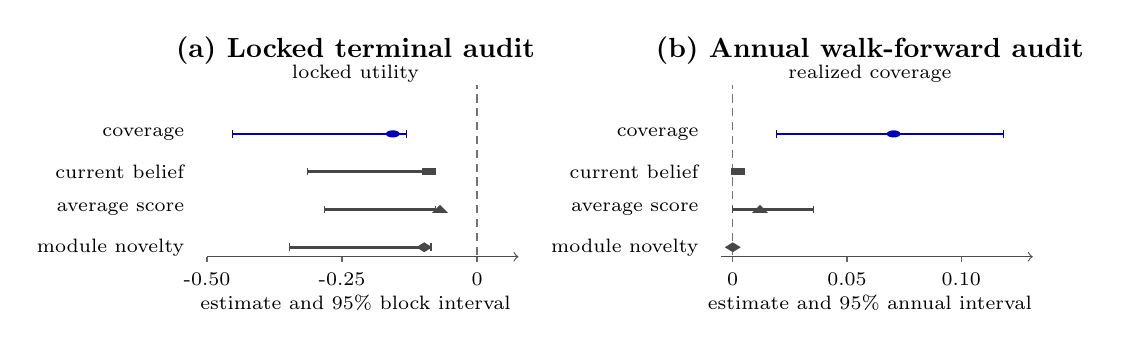
\begin{tikzpicture}[x=0.92cm,y=0.48cm,font=\scriptsize]
  \node[font=\bfseries] at (4.05,5.45) {(a) Locked terminal audit};
  \node at (4.05,4.85) {locked utility};
  \node[font=\bfseries] at (11.15,5.45) {(b) Annual walk-forward audit};
  \node at (11.15,4.85) {realized coverage};
  \draw[black!55,densely dashed] (5.727273,0.05) -- (5.727273,4.55);
  \draw[black!55,densely dashed] (9.257692,0.05) -- (9.257692,4.55);
  \draw[blue!72!black,line width=0.9pt] (2.349676,3.25) -- (4.757297,3.25);
  \draw[blue!72!black] (2.349676,3.15) -- (2.349676,3.35);
  \draw[blue!72!black] (4.757297,3.15) -- (4.757297,3.35);
  \fill[blue!72!black] (4.564722,3.25) circle (0.095);
  \node[anchor=east] at (1.82,3.25) {coverage};
  \draw[black!72,line width=0.9pt] (3.387103,2.25) -- (5.148218,2.25);
  \draw[black!72] (3.387103,2.15) -- (3.387103,2.35);
  \draw[black!72] (5.148218,2.15) -- (5.148218,2.35);
  \fill[black!72] (4.973837,2.16) rectangle (5.153837,2.34);
  \node[anchor=east] at (1.82,2.25) {current belief};
  \draw[black!72,line width=0.9pt] (3.624146,1.25) -- (5.155993,1.25);
  \draw[black!72] (3.624146,1.15) -- (3.624146,1.35);
  \draw[black!72] (5.155993,1.15) -- (5.155993,1.35);
  \fill[black!72] (5.216539,1.37) -- (5.106539,1.16) -- (5.326539,1.16) -- cycle;
  \node[anchor=east] at (1.82,1.25) {average score};
  \draw[black!72,line width=0.9pt] (3.141269,0.25) -- (5.092602,0.25);
  \draw[black!72] (3.141269,0.15) -- (3.141269,0.35);
  \draw[black!72] (5.092602,0.15) -- (5.092602,0.35);
  \fill[black!72] (4.997946,0.38) -- (4.887946,0.25) -- (4.997946,0.12) -- (5.107946,0.25) -- cycle;
  \node[anchor=east] at (1.82,0.25) {module novelty};
  \draw[blue!72!black,line width=0.9pt] (9.855796,3.25) -- (13.00087,3.25);
  \draw[blue!72!black] (9.855796,3.15) -- (9.855796,3.35);
  \draw[blue!72!black] (13.00087,3.15) -- (13.00087,3.35);
  \fill[blue!72!black] (11.478529,3.25) circle (0.095);
  \node[anchor=east] at (8.92,3.25) {coverage};
  \draw[black!72,line width=0.9pt] (9.257692,2.25) -- (9.41809,2.25);
  \draw[black!72] (9.257692,2.15) -- (9.257692,2.35);
  \draw[black!72] (9.41809,2.15) -- (9.41809,2.35);
  \fill[black!72] (9.226471,2.16) rectangle (9.406471,2.34);
  \node[anchor=east] at (8.92,2.25) {current belief};
  \draw[black!72,line width=0.9pt] (9.257692,1.25) -- (10.368312,1.25);
  \draw[black!72] (9.257692,1.15) -- (9.257692,1.35);
  \draw[black!72] (10.368312,1.15) -- (10.368312,1.35);
  \fill[black!72] (9.633211,1.37) -- (9.523211,1.16) -- (9.743211,1.16) -- cycle;
  \node[anchor=east] at (8.92,1.25) {average score};
  \draw[black!72,line width=0.9pt] (9.257692,0.25) -- (9.257692,0.25);
  \draw[black!72] (9.257692,0.15) -- (9.257692,0.35);
  \draw[black!72] (9.257692,0.15) -- (9.257692,0.35);
  \fill[black!72] (9.257692,0.38) -- (9.147692,0.25) -- (9.257692,0.12) -- (9.367692,0.25) -- cycle;
  \node[anchor=east] at (8.92,0.25) {module novelty};
  \draw[->,black!70] (2.0,0) -- (6.3,0);
  \draw[->,black!70] (9.1,0) -- (13.4,0);
  \foreach \value/\label in {-0.5/{-0.50},-0.25/{-0.25},0/{0}} {
    \pgfmathsetmacro{\xp}{2.0+4.1*(\value+0.5)/0.55}
    \draw[black!60] (\xp,0) -- (\xp,-0.13);
    \node[anchor=north] at (\xp,-0.18) {\label};
  }
  \foreach \value/\label in {0/{0},0.05/{0.05},0.10/{0.10}} {
    \pgfmathsetmacro{\xp}{9.1+4.1*(\value+0.005)/0.13}
    \draw[black!60] (\xp,0) -- (\xp,-0.13);
    \node[anchor=north] at (\xp,-0.18) {\label};
  }
  \node[anchor=north] at (4.05,-0.75) {estimate and 95\% block interval};
  \node[anchor=north] at (11.15,-0.75) {estimate and 95\% annual interval};
\end{tikzpicture}

  \caption{Secondary coverage-ranking estimands on separate audit-specific
  axes: held-out locked-utility change in the terminal audit and next-year
  realized set coverage in the annual audit.  Points and 95\% intervals are
  rendered floating-point summaries from the committed resampling rows, not
  exact rationals.  The terminal outcome is adverse; the annual outcome is
  supportive but noisy, with only five annual target units.  The descriptive
  intervals do not cover design uncertainty.}
  \label{fig:supp-financial-coverage-comparison}
\end{figure}

These audits are retrospective mechanism evidence.  They support no causal,
forecasting, alpha, or deployable-performance claim.
